\subsection{Orientering}

Dette afsnit beskriver test af dronens orientering. 

Dronen skal have den rette orientere, før den kan flyve fremad. For at finde orienteringen, bruges 3G/GPS modulet, kompas og main controlleren.

Til testen af orientering er nuværende og ønskede GPS positioner hardcoded. 
Den nuværende og ønskede GPS positions sammenlignes og orienteringen findes. Fra kompasset aflæser main controlleren dronens orientering og sammenligner med den ønskede orientering. Hvis orienteringerne ikke er ens, skal dronen ændre retning, retningen ændres ved at forøge eller formindske Yaw parameteren. 
På figur \ref{fig:orientering_skift} vises hvad main controlleren gør. Main controlleren sammenligner nuværende med ønskede orientering, hvis orienteringen ikke er indenfor det ønskede interval, ændres denne.

\begin{figure}[H]
\centering
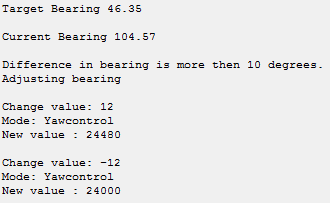
\includegraphics[width=0.5\textwidth]{Billeder/Test/bearing_test.png}
\caption{Ændring af orientering}
\label{fig:orientering_skift}
\end{figure}

Hvis orienteringen er indenfor intervallet, vil outputtet være som på figur \ref{fig:orientering_interval}.

\begin{figure}[H]
\centering
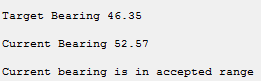
\includegraphics[width=0.4\textwidth]{Billeder/Test/bearing_reached.png}
\caption{Orientering er i intervallet}
\label{fig:orientering_interval}
\end{figure}